\chapter{Related Work}

\section{ROS}
The Robot Operating System (ROS) is an Open Source framework for complex robotic systems. The first work on ROS was done as part of the STanford Artificial Intelligence Robot (STAIR) in 2007 \cite{Quigley2007}. The original software library was called \emph{Switchyard} and had been developed at Stanford. Later the library was refined and generalized to also suit the requirements of the Personal Robot Program at Willow Garage\footnote{www.willowgarage.com} \cite{Quigley2009}. The resulting general framework has been released as Open Source \cite{Quigley2009} and this section gives a short overview over the most important principles in ROS.

\begin{figure}[ht]
\centering
\subfigure[Stanford's STAIR]{
	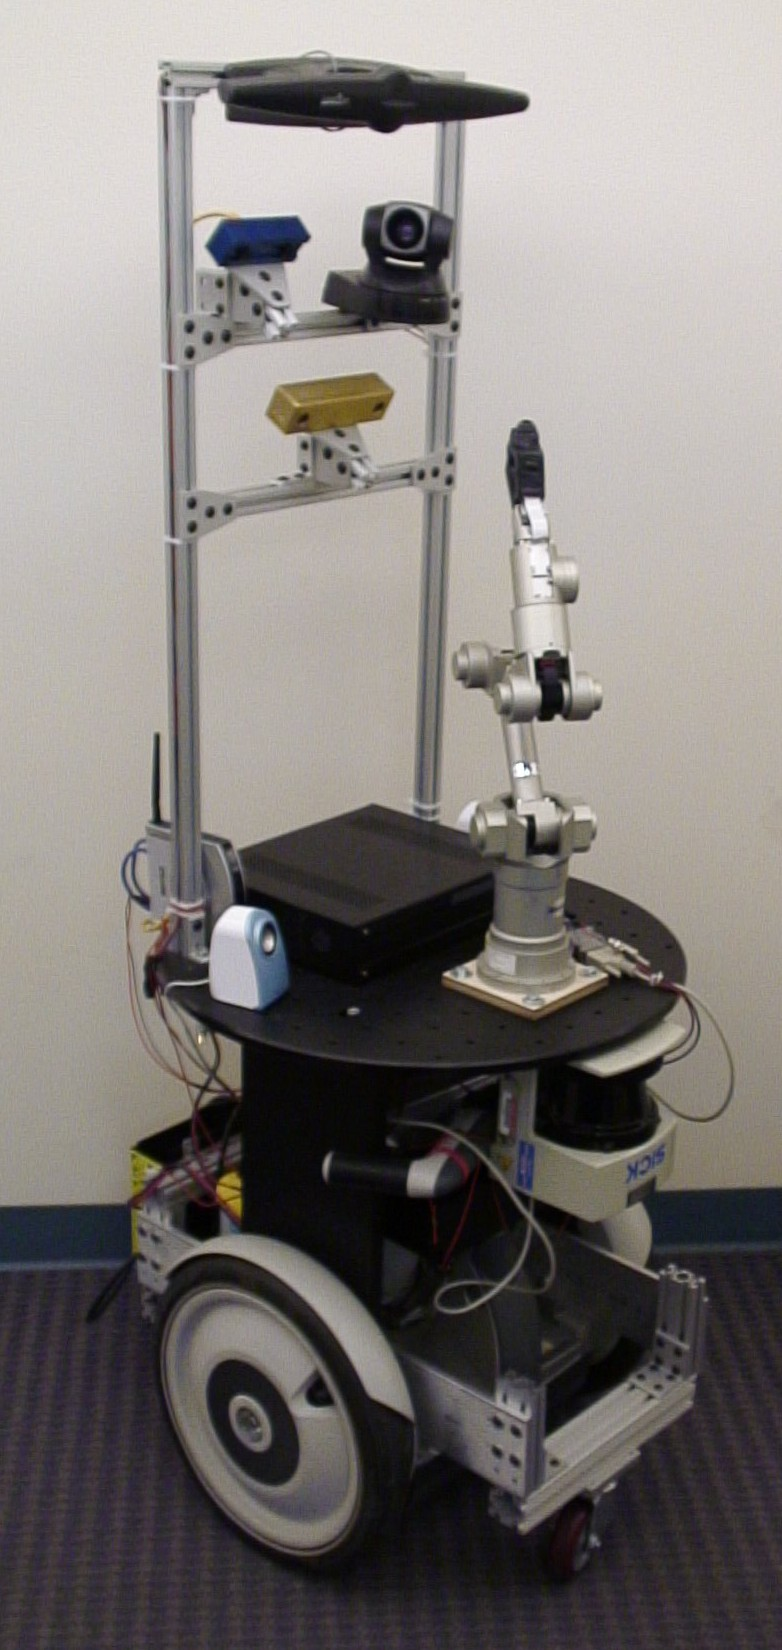
\includegraphics[height=8cm]{img/stair}
}
\subfigure[Willow Garage's PR2]{
	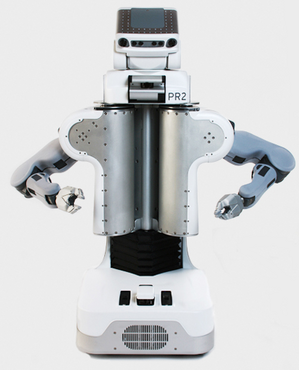
\includegraphics[height=8cm]{img/pr2}
}
\end{figure}

ROS was built to abstract from the hardware of the robot and create modular robot software, which can run on different robots and on different machines. This makes it easier to write software for robots and distribute the work to different teams, each team focusing on one part of the robot. The modules in ROS are called nodes and several nodes executed together are called a stack. ROS packages bundle nodes and stacks and are used to make software modules available to other developers. Everyone can create their own package which can be indexed by ROS so that your software modules can be found, downloaded and used by other developers. There exist many packages, nodes and stacks for some of the most common problems in robotics, which can easily be re-used: navigation, localization, movement, etc.

The communication between ROS nodes can be done asynchronously through a publish/subscribe mechanism and synchronously through services. Nodes can send messages by publishing a message on a topic and receive messages by subscribing to that topic. This mechanism is really flexible and decouples the sender from the receiver. A publisher node does not need to know if there are other nodes listening and vice versa. For synchronous communication and guaranteed delivery of messages, services can be invoked. The routing is established during runtime through the ROS core. The core of ROS was kept really slim and only contains the most essential parts of the framework (such as the inter node communication). ROS can run on several machines distributed in a network, the only restriction is that every node needs to know the address of the core (master node) in order to communicate with other nodes.

A variety of tools have been built around the ROS core to facilitate the development of ROS nodes and robotic software in general. The philosophy for those tools is to be small and do one job only but do it good. The result are really robust tools similar to the toolchain available on Linux. The downside is a big variety of tools in the ROS ecosystem, which can be confusing to new developers.

The latest stable version of the ROS framework was released in April 2012 (ROS Fuerte). Previous releases of stable versions have been in August 2011 (ROS Electric), March 2011 (ROS Diamondback), August 2010 (ROS C Turtle) and March 2010 (ROS Box Turtle). There are currently many institutions, companies and individuals involved in the ROS community, contributing in many different ways.

\section{Tracepoints}
\section{rxDeveloper}
\section{Other Debugging Work}
